%%
%% Author: maximelovino
%% 2019-06-24
%%

% Preamble
\documentclass[11pt]{article}
\setlength{\parindent}{0pt}
\addtolength{\hoffset}{-3cm}
\addtolength{\textwidth}{6cm}

\addtolength{\voffset}{-2cm}
\addtolength{\textheight}{4cm}

% Packages
\usepackage{amsmath}
\usepackage{url}
\usepackage{graphicx}
\usepackage{float}
\usepackage[T1]{fontenc}
\usepackage[utf8]{inputenc}
\title{Wikipedia Web Traffic Forecasting\\Machine Learning on Big Data - HES-SO Master}
\author{Maxime Alexandre Lovino \and Marco Rodrigues Lopes}

% Document
\begin{document}
    \maketitle
    \section{Introduction and project description}
    This project is inspired by a competition posted by Google on Kaggle\footnote{\url{https://www.kaggle.com/c/web-traffic-time-series-forecasting/}} and is based around the idea of forecasting time series values. For this project, we drew inspirations by submissions from other competitors on Kaggle as well as the work of \emph{JEddy92} on GitHub\footnote{\url{https://github.com/JEddy92/TimeSeries_Seq2Seq}} which inspired our use of the WaveNet model for this project.\\

    Time series are used in multiple domains, the most well known being the stock market values, so we could apply the same type of models to predict stock market changes and become rich....But in practice it would actually be more efficient to use external factors such as trending topics or news articles to find correlations with the changes in the time series.\\

    In this project, we didn't have only one time series to predict but actually a lot of them. 145000 different time series were provided spanning 2.5 years with a granularity of 1 day. The goal of the project is to predict the values for each of them for 60 days in the future. For this project, we didn't use external data to help us with the predictions and relied solely on the time series themselves to predict future values.\\

    In order to respect the maximum number of pages specified for this report, we will only discuss models, techniques and results from our best model(s) and will discuss discarded ones shortly during the oral presentation.
    \newpage
    \section{Data description}
    The dataset that can be downloaded on Kaggle consists of two training files in the CSV format and other files which are not relevant to our problem as they're only used for actually submitting an answer for the competition. The two training files consists of the same set of 145000 pages and the same starting date but the second one:\verb+train_2.csv+ is longer, spanning almost 803 days. We decided to use the longer for our experiment has it contains at least two complete years of data. The CSV file weighs 400 MB uncompressed.\\

    The structure of the file consists of a first column containing the page information concatenated in a string, with the title of the page, the lang, the access type and the agent and then a column for each day with the number of views that the specific page got on that day. Some page have \verb+NaN+ values for view on certain dates and this corresponds to the page not having been created yet on that date or just missing values.

    \begin{figure}[H]
        \centering
        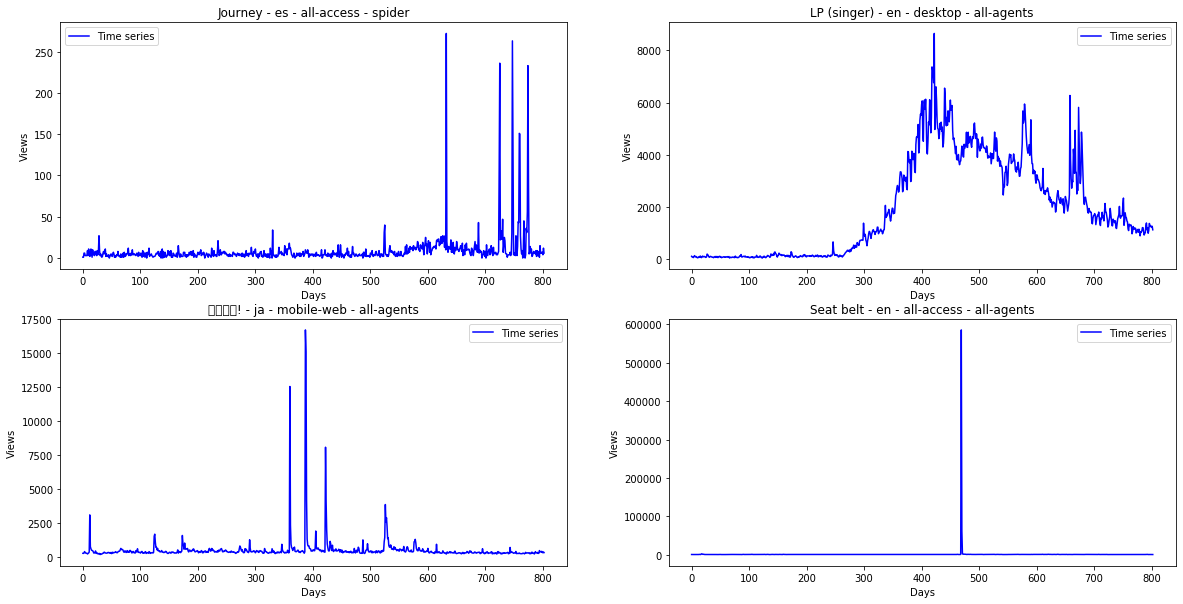
\includegraphics[width=\textwidth]{pages.png}
        \caption{Some of the pages present in the dataset}
    \end{figure}
    \section{Data cleaning and pre-processing}
    The preprocessing and cleaning of the CSV file is handled in the \verb+preprocess_csv_to_pickle+ static method of the \verb+WikiSeries+ classes we have created. This will take a CSV file as an input, extract the information contained in the first column to split in 4 columns (title, lang, access, agent) and remove any page which doesn't belong to a specific country Wikipedia subdomain\footnote{Wikimedia for example}. We will also remove all pages containing \verb+NaN+ values in their series as we can't really replace them with 0 because they didn't actually get 0 views as they didn't exist so we removed them to only work with clean data. After all these steps, we save the resulting Dataframe as a Pickle which will then be used by our other programs. With this cleaning, we reduced our number of pages from 145’063 pages down to 106'328 pages.
    \newpage
    \section{Machine Learning techniques used}
    \subsection{Walk forward validation}
    Before training our models, we had to decide how we wanted to split our data. Splitting by pages doesn't make a lot of sense for time series so instead we decided to use Walk Forward validation so that we evaluate the same pages but for a different 60-days windows when evaluating our models. When specifically fitting the model though, we took 40'000 pages and dedicated 20\% for Keras validation so we used a side by side split to fit the model.
    \begin{figure}[H]
        \centering
        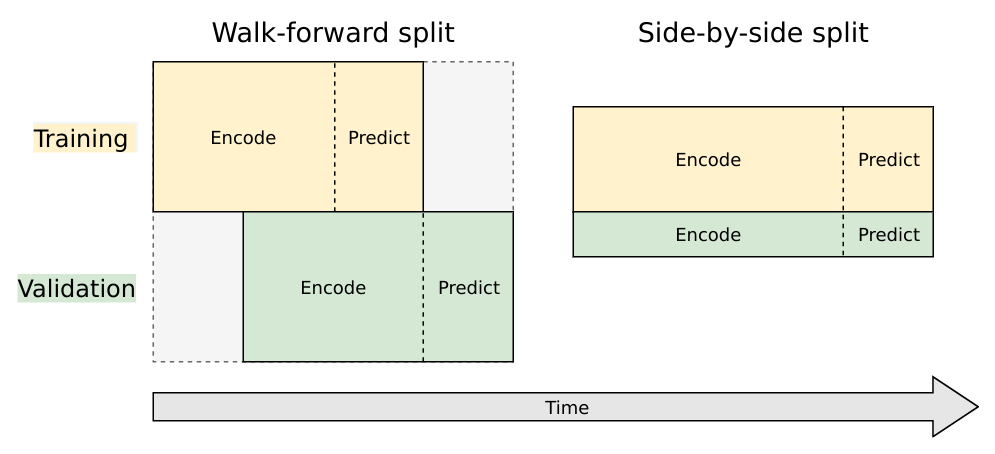
\includegraphics[width=.7\textwidth]{walkforward.png}
        \caption{Walk forward validation}
    \end{figure}
    \subsection{Data normalisation}
    We normalise data using \verb+log1p+, that is $log(x+1)$ as well as removing the mean of the series from all page normalised page views. After predicting, we do the inverse transformation before displaying results and computing metrics.

    \subsection{Seq2Seq models}
    The idea behind Seq2Seq is that we have an encoder and a decoder. This model was created by Google for translating text. The foreign language text would be fed as the encoder with the list of words in the foreign language and then fed to the decoder with translated words chained in the decoder. In our context, the encoder is the historical time series data on which we are training the model and the decoder is the predicted data for the future. Seq2Seq models are based on LSTM\footnote{Long short term memory} layers that will surface old information at a later stage in order to not only fit on the most recent information in the encoder. We use teacher forcing during training by putting the decoder target in the encoder as well so that the fitting of the model can use the target value to find the next one and compare to the expected decoder.
    \begin{figure}[H]
        \centering
        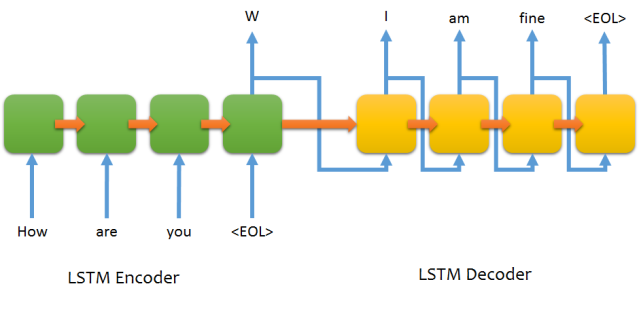
\includegraphics[width=.6\textwidth]{seq2seq.png}
        \caption{Seq2Seq models}
    \end{figure}
    \subsection{WaveNet}
    WaveNet is another model developed by DeepMind\footnote{DeepMind is actually Google}, this time for text-to-speech application. The idea here is that we will use convolutional layers to combine inputs from different encoder steps. In our case, we use causal dilational convolutions, so that in each hidden layer, we combine further apart steps (exponentially up to $log_2(days)$ distance between steps) in a causal manner, meaning that we only combine forward and not backward. This in the end leads to the output being a combination of values from 2, 4, 8, 16,... days before. The main difference in our implementation is that we use a \verb+ReLu+ activation instead of a \verb+SoftMax+ as we want to predict a continuous value and not a categorical one.\\

Our full WaveNet model has 2 * 10 convolutional layers (increasing then decreasing step sizes) multiplied together with \verb+tanh+ and \verb+sigmoid+ activations (gated activation) with residual and skip connections.
    \begin{figure}[H]
        \centering
        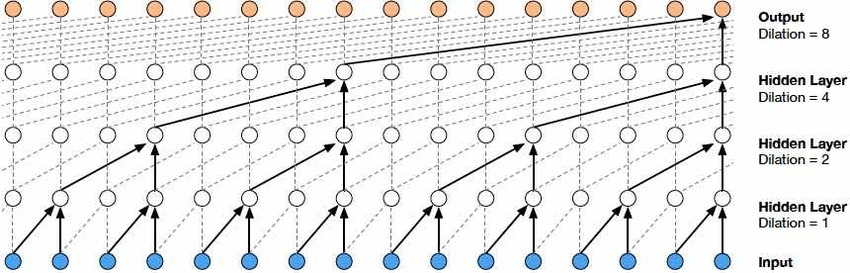
\includegraphics[width=.6\textwidth]{wavenet.jpg}
        \caption{WaveNet causal dilation}
    \end{figure}
    \newpage
    \section{Experiments and results}
    \subsection{Training in the cloud}
    We had to use cloud infrastructures, such as Google Cloud and Amazon AWS in order to train our models on big GPUs in a reasonable time. We mainly used Tesla K80 cards on Google Cloud as well as some Tesla V100 cards from Nvidia. Our more complex model, the full WaveNet with the most layers, skips and residuals took 2 minutes per epoch to train.\\

    Evaluating prediction for all 100'000 time series took a long time as well, we did it in batches but it still took more or less 20 minutes on those same GPUs for the most complex model.
    \subsection{Evaluating results with SMAPE}
    The metric we used to evaluate our results was the SMAPE\footnote{Symmetric Mean Absolute Percentage Error} which was used in the Kaggle competition. The SMAPE provides a relative error so that errors in pages with a high number of views won't influence our results more than errors on small pages. The formula used to compute the SMAPE is the following\footnote{This gives directly the percentage value, so a result of 35 means a 35\% SMAPE value}:
    \begin{equation*}
        \frac{100\%}{days} * \sum_{t=0}^{t=days}\frac{2 * |\hat{y}_t-y_t|}{|y_t| + |\hat{y}_t|}
    \end{equation*}
    \subsection{Results for single day predictions}
    We evaluated at first for single day prediction, that means that for each day $t$, we inserted the target $y_{t-1}$ as last step for the prediction. With this we obtained SMAPE values of 24.885\% for the simple WaveNet and 23.708\% for the full one.
    \subsection{Results for 60 days prediction}
    Then we evaluated for the full 60 days, that means that for each day $t$, we inserted the prediction $\hat{y}_{t-1}$ as last step for the prediction. With this we obtained SMAPE values of 37.2910\% for the simple WaveNet and 34.6499\% for the full one. This last result is impressive as it is better than the result from the winner of the competition. However, the results were not computed on the same period as the period used for computing results has never been published and also our result has only been computed on pages containing non \verb+NaN+ values.
    \begin{figure}[H]
        \centering
        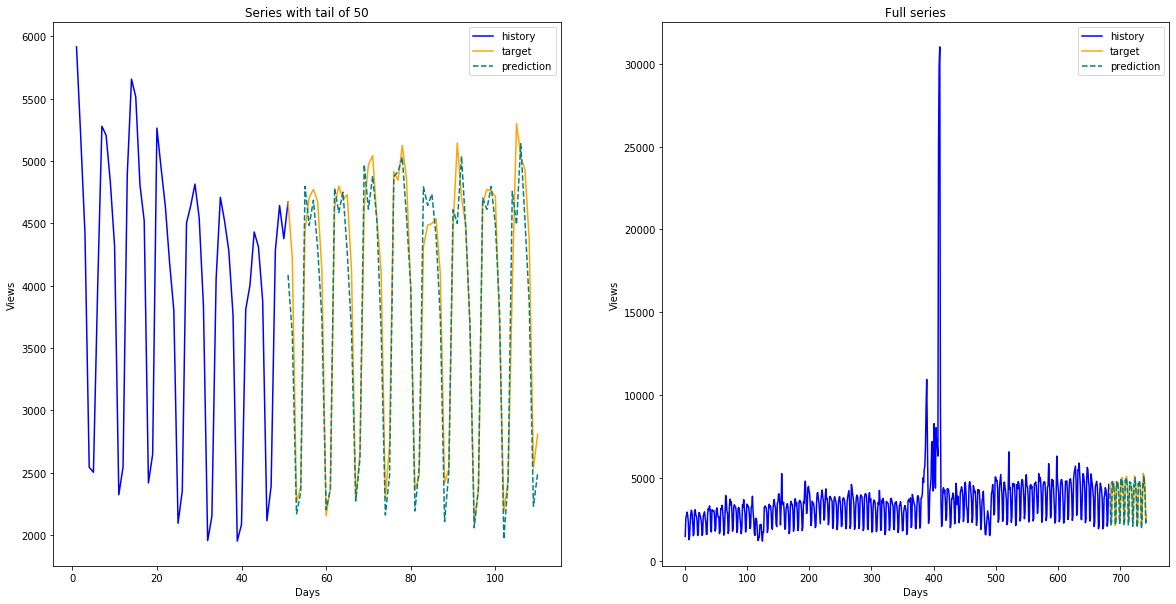
\includegraphics[width=\textwidth]{prediction_single.png}
        \caption{Single day prediction for Wikipedia EN Main page}
    \end{figure}
    \begin{figure}[H]
        \centering
        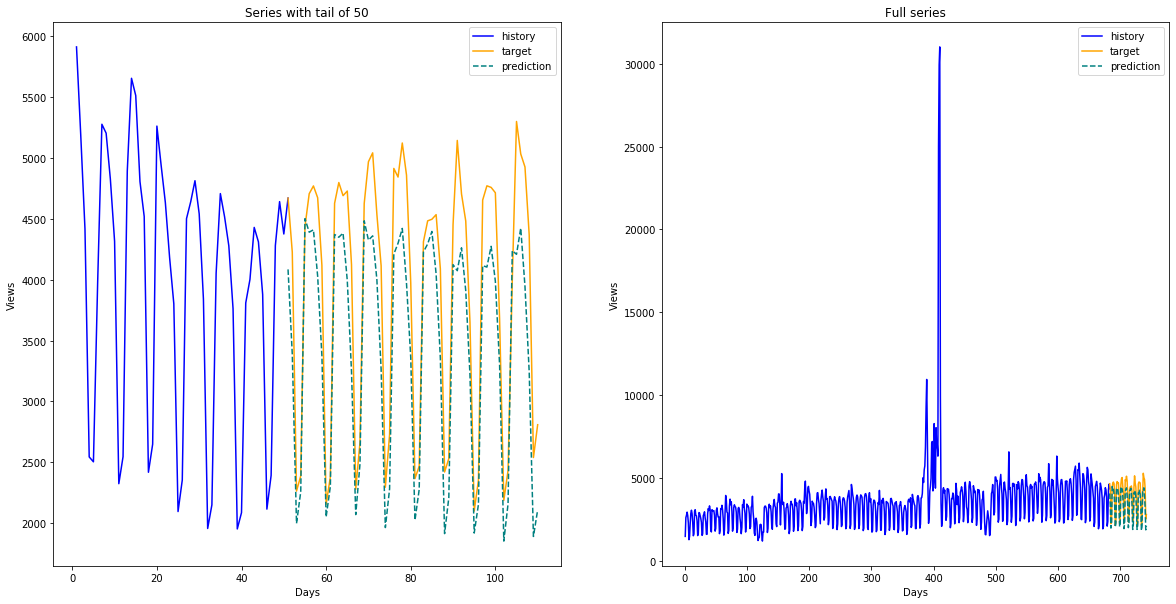
\includegraphics[width=\textwidth]{prediction.png}
        \caption{60 days prediction for Wikipedia EN Main page}
    \end{figure}
    \newpage
    \section{Analysis and conclusions}
We really enjoyed working on this project as it allowed us to learn a lot about time series and deep learning models, in particular Seq2Seq and WaveNet. We discovered a lot of concepts such as teacher forcing, walk forward validation that we didn't really see in class as we didn't have a full chapter on time series or specific deep learning models. It would have been easier if we had seen Seq2Seq models or even LSTM before in class. \\

    As always with deep learning, we actually used existing models that we adapted to our problem, but we still managed to understand how they worked and grasp the concepts behind them. For the kinds of problems we handled in this project, we can't really avoid using deep learning models as they provide the best results and they take advantages of GPUs to be trained in reasonable time. Also, we often don't need to extract a lot of features, often categorical, as it is often the case with classic models. This feature extraction can often take even more time than the training itself and in our case led to explosion of memory and CPU usages without providing good results.\\

    As far as the obtained results are concerned, we actually managed to beat the competition winner, although we removed problematic series in our case, which left us really impressed with the power of the relatively simple to code model we created. By using Keras, we can build a complex models in really few lines of code.\\

    For the scope of the project, the most useful predictions though would be the one day predictions in our opinion as most sites are hosted on cloud infrastructures and predicting one traffic one day in advance would already provide enough time to scale infrastructure proactively instead of reactively thus providing a better experience for site users.\\


\end{document}